\section{Evaluation}
%TODO: Is there a good technical reason why every \absmachine machine
% should have exactly one large stateful atom as opposed to many small stateful atoms?
% TODO: Show how pipeline width / depth changes
% by adding more complicated atoms? This might be a little more work though.
\label{s:eval}

\begin{table}[!t]
  \begin{scriptsize}
  \begin{tabular}{|p{0.1\textwidth}|p{0.35\textwidth}|}
    \hline
    Atom & Description \\
    \hline
    Write & Write packet field/constant into single state variable. \\
    \hline
    ReadAddWrite (RAW) & Add packet field/constant to state variable (OR) Write packet field/constant into state variable. \\
    \hline
    Predicated ReadAddWrite (RAW) & Execute RAW on state variable only if a predicate is true, else leave unchanged. \\
    \hline
    IfElse ReadAddWrite (IfElseRaw) & Execute two separate RAWs: one each for when a predicate is true or false.\\
    \hline
    Subtract (Sub) & Same as IfElseRaw, but also allow subtracting a packet field/constant. \\
    \hline
    Nested Ifs (Nested) & Same as Sub, but with an additional level of nesting that provides 4-way predication. \\
    \hline
    Paired updates (pairs) & Same as Nested, but allow updates to a pair of state variables, where predicates can use both state variables. \\
    \hline
  \end{tabular}
  \end{scriptsize}
  \caption{Atoms used in evaluation. Appendix A provides the SKETCH code and
  circuit diagrams for these atoms.}
  \label{tab:templates}
\end{table}

\begin{table}[!t]
  \begin{scriptsize}
    \begin{tabular}{|p{0.08\textwidth}|p{0.3\textwidth}|p{0.03\textwidth}|}
  \hline
  Atom & Circuit & Circuit depth \\
  \hline
  Write & 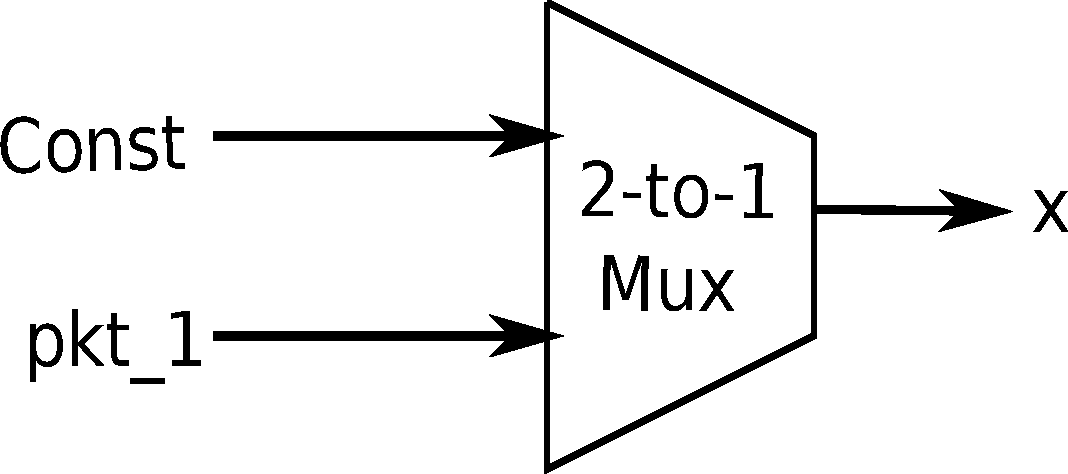
\includegraphics[width=0.2\textwidth]{rw.pdf} & 1 \\
  \hline
  ReadAddWrite (RAW) & 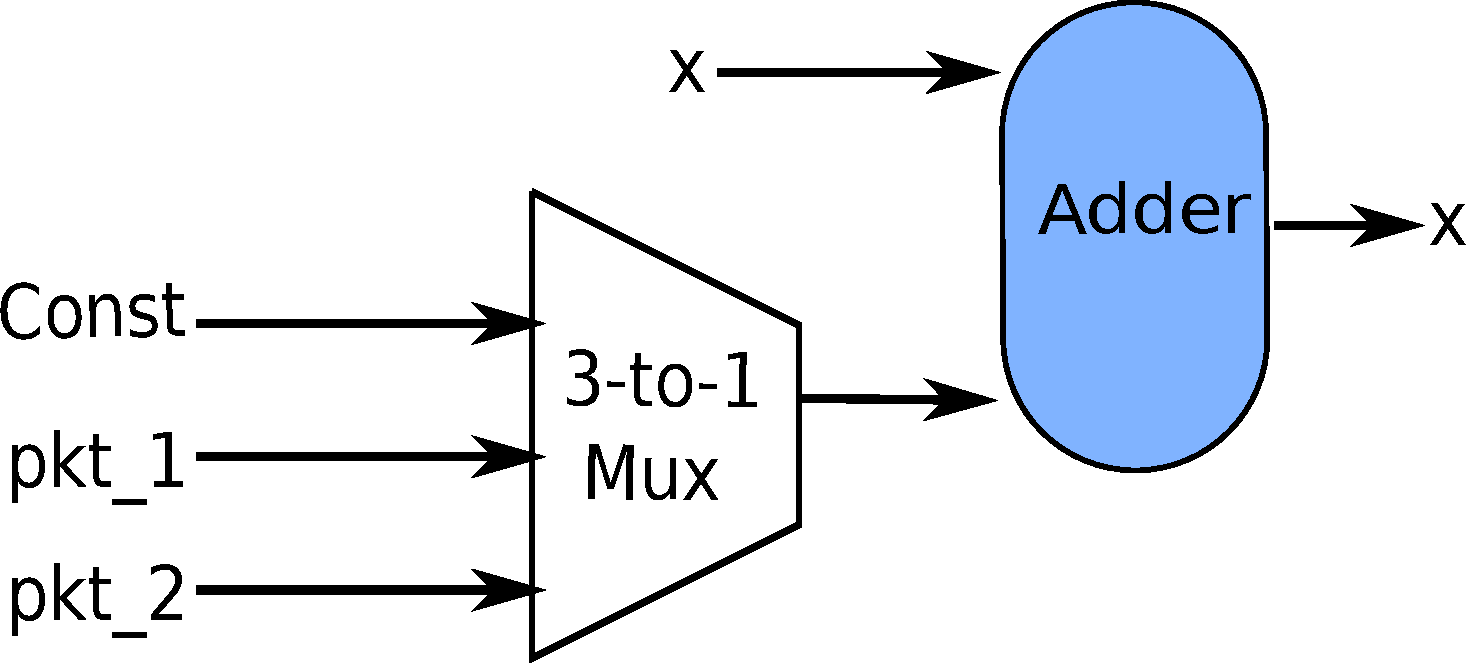
\includegraphics[width=0.2\textwidth]{raw.pdf} & 2\\
  \hline
  \pbox{0.1\textwidth}
  {Predicated\\
  ReadAddWrite (PRAW)} & 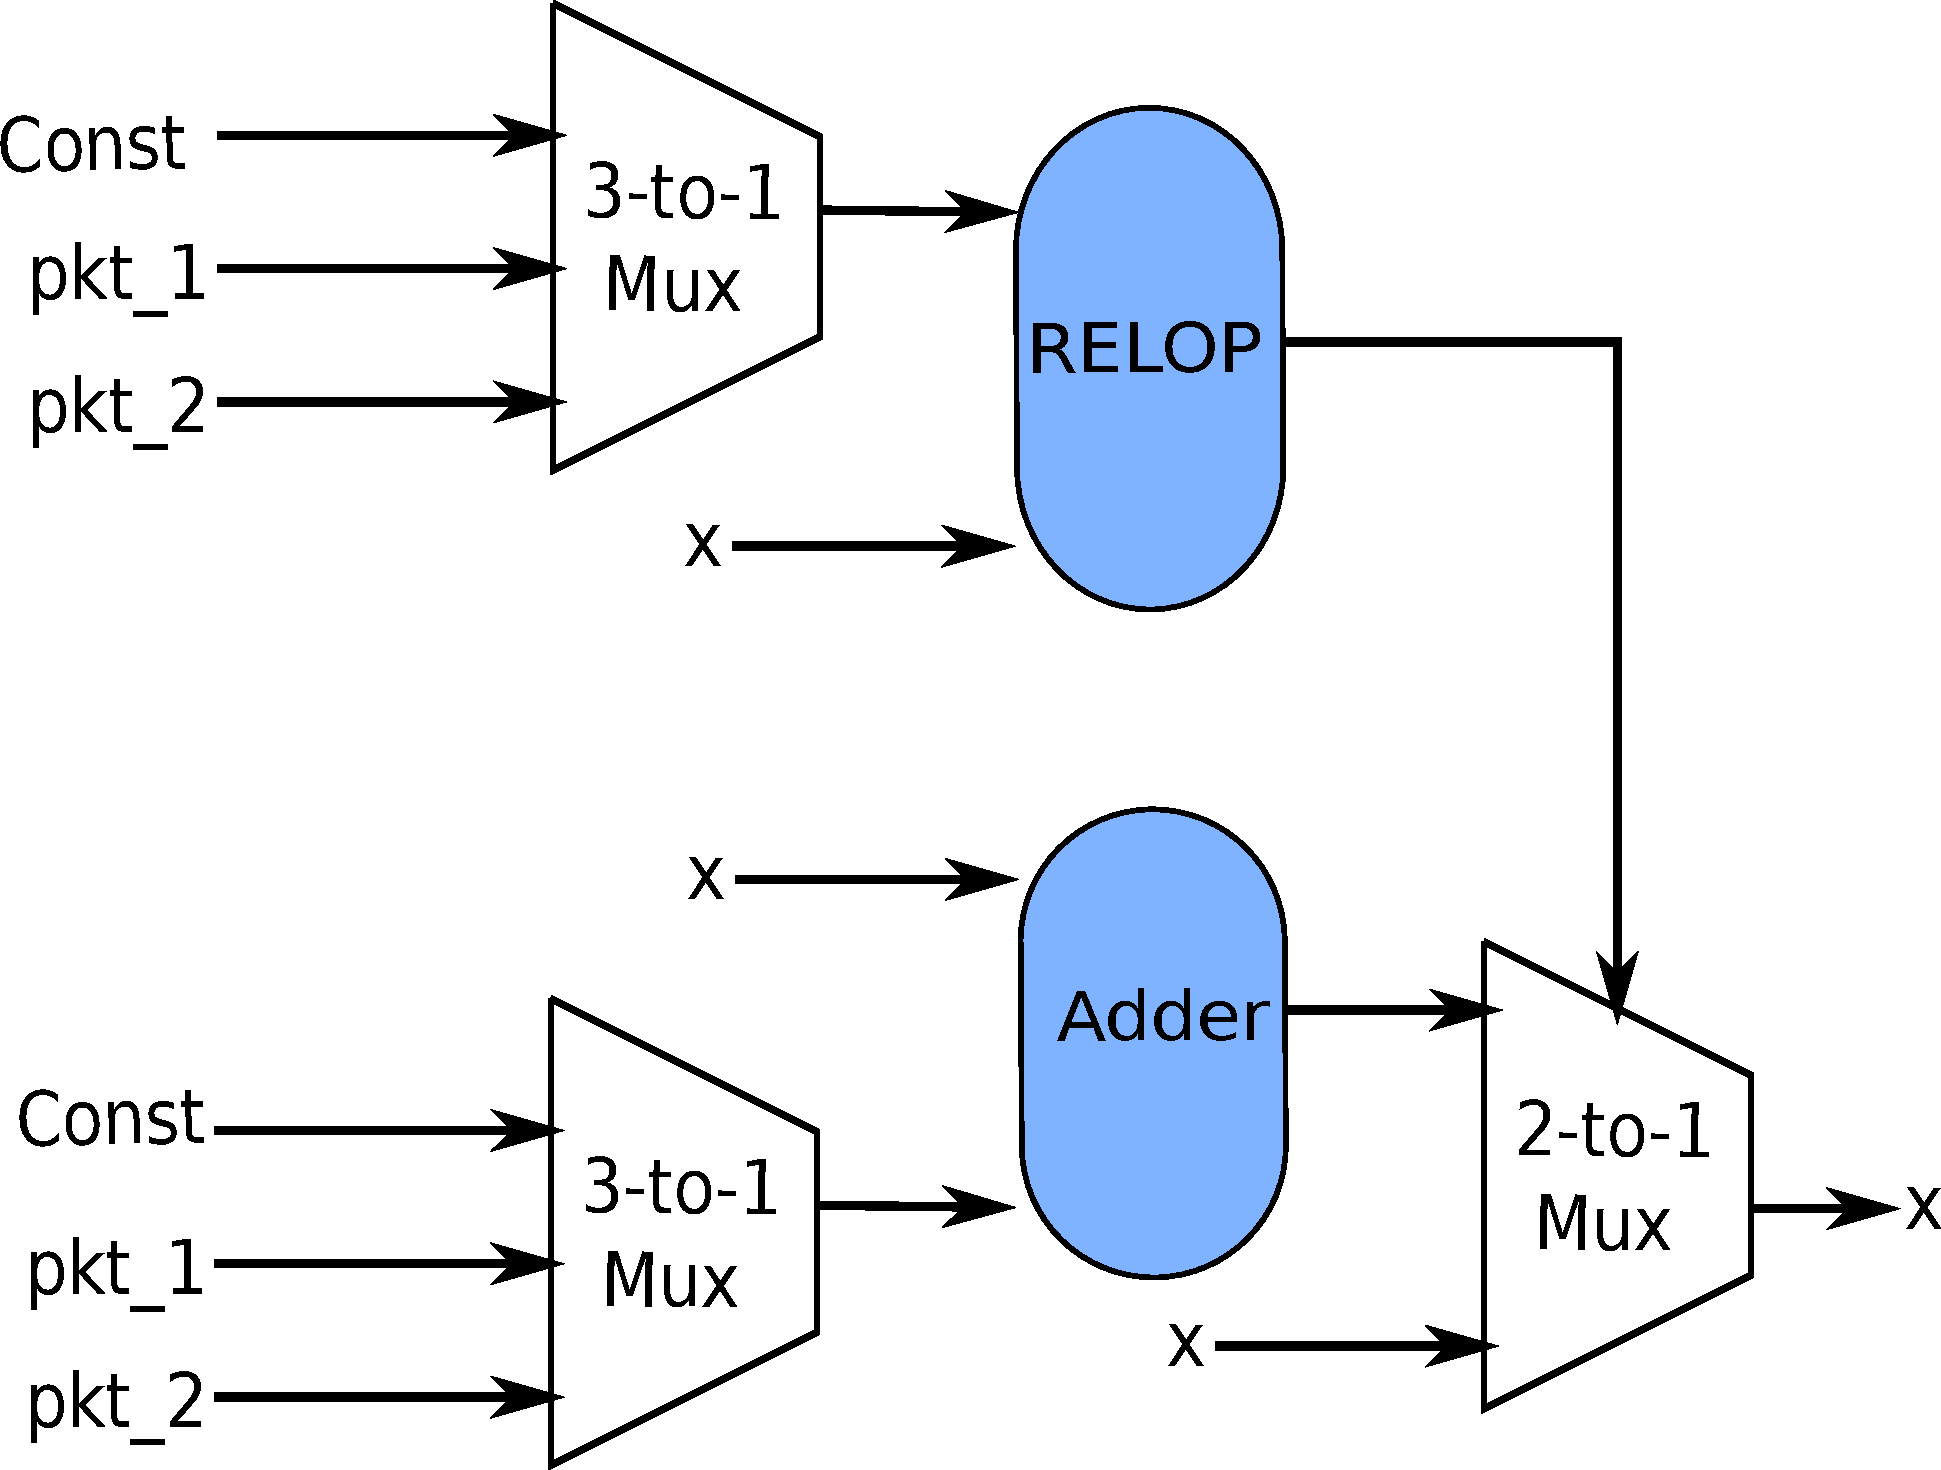
\includegraphics[width=0.3\textwidth]{pred_raw.pdf}  & 3\\
  \hline
  \end{tabular}
\end{scriptsize}
\caption{Circuit depth and propagation delay increases with complexity of atoms.}
  \label{tab:circuit_depth}
\end{table}

\begin{table*}[!t]
  \begin{tabular}{|p{0.16\textwidth}|p{0.47\textwidth}|p{0.10\textwidth}|p{0.5\textwidth}|p{0.5\textwidth}}
\hline
Algorithm & Stateful computation & Least expressive atom & Pipeline depth & Pipeline width \\
\hline
Bloom filter~\cite{bloom} & \pbox{0.54\textwidth}{Set membership bit on every packet.} & Write & 4 & 3\\
\hline
Heavy Hitters~\cite{opensketch} & Increment Count-Min Sketch~\cite{cormode} on every packet. & RAW & 10 & 9 \\
\hline
Flowlets~\cite{flowlets} & Update saved next hop if flowlet threshold is exceeded. & PRAW & 6 & 3 \\
\hline
RCP~\cite{rcp} & \pbox{0.54\textwidth}{Accumulate RTT sum if\\RTT is under maximum allowable RTT.} & PRAW & \\
\hline
Sampling & \pbox{0.54\textwidth}{Sample/Mark a packet if packet count reaches N;\\Reset count to 0 when it reaches N.} & If-Else RAW &\\
\hline
HULL~\cite{hull} & Update counter for virtual queue. & Sub & \\
\hline
AVQ~\cite{avq} & Update virtual queue size and virtual capacity & Nested & \\
\hline
CONGA~\cite{conga} & \pbox{0.54\textwidth}{Update best path's utilization/id if we see a better path.\\
                                           Update best path utilization alone if it changes.}  & Pairs & \\
\hline
trTCM~\cite{trTCM} & Update token counts for each token bucket & Doesn't map & \\
\hline
CoDel~\cite{codel} & \pbox{0.54\textwidth}{Update:\\Whether we are dropping or not.\\Time for next drop.\\Number of drops so far.\\Time at which min. queuing delay has exceeded target.}& Doesn't map & \\
\hline
\end{tabular}
\caption{Data-plane algorithms}
\label{tab:algos}
\end{table*}

To evaluate \pktlanguage, we express several data-plane algorithms
(Table~\ref{tab:algos}) using \pktlanguage and determine if they are
implementable on different \absmachine machines that provide different stateful
atoms (Table~\ref{tab:templates}). Appendix A contains circuit diagrams and
SKETCH code for each of these atoms.

\subsection{Experimental procedure}
As mentioned in \S\ref{ss:code_gen}, we consider only stateful atoms by
assuming stateless codelets map one-to-one to stateless atoms for all
\absmachine machines. For simplicity, the stateful atoms only permit updates to
state variables and forbid packet field updates mixed in with these state
updates.  Assuming the \absmachine machine provides an atom to read a state
variable\footnote{The inability to read a state variable renders it
powerless!}, such packet updates can be treated as stateless operations in
subsequent pipeline stages.

We also assume every \absmachine machine provides exactly one stateful atom.
Table~\ref{tab:templates} gradually increases the capability of this single
atom.  We designed the atoms in Table~\ref{tab:templates}, and hence the
\absmachine machines providing them, to form a containment hierarchy: each atom
can express all data-plane algorithms that its predecessor can.

We now consider every atom/\absmachine machine from Table~\ref{tab:templates},
and every data-plane algorithm from Table~\ref{tab:algos} to determine if each
algorithm is \textit{implementable} on a particular \absmachine machine. We say
an algorithm is implementable on a \absmachine machine, if every stateful
codelet within the data-plane algorithm can be mapped (\S\ref{ss:code_gen}) to
the single stateful atom provided by the \absmachine machine. Because atoms are
arranged in a containment hierarchy, we list the \textit{least expressive} atom
that can be used to implement a data-plane algorithm in Table~\ref{tab:algos}.

% At this point now ....
%
%\subsection{Interpreting these results}
%Figure~\ref{fig:eval} tells a network programmer if a particular data-plane
%algorithm can be implemented at line rate, assuming the \absmachine machine
%provides a particular stateful atom. For an ASIC engineer designing
%programmable switching chips, the same figure describes the algorithms that are
%implementable on a particular \absmachine machine. For instance, a \absmachine
%machine with the paired updates atom can implement eight algorithms shown in
%Figure~\ref{fig:eval}, while a machine with a simpler read-add-write atom can
%implement only two.
%
%These results will change as programmable switches evolve and network
%programmers push chip boundaries with new algorithms.  The larger takeaway is
%that programming in \pktlanguage allows us to rigorously determine if a
%particular high-level algorithm is implementable at line rate on a particular
%\absmachine machine. Conversely, it tells us if a particular \absmachine
%machine suffices to implement a large number of algorithms.
%
%\subsection{Compilation times}
